% Sample file on how to use subfiles.
\documentclass[ExampleMasters.tex]{subfiles}

\begin{document}
\clearpage
\appendix 
\addcontentsline{toc}{chapter}{APPENDICES}

\chapter{Appendix}
\label{chap:Appendix}

\begin{figure}[h]
\centering
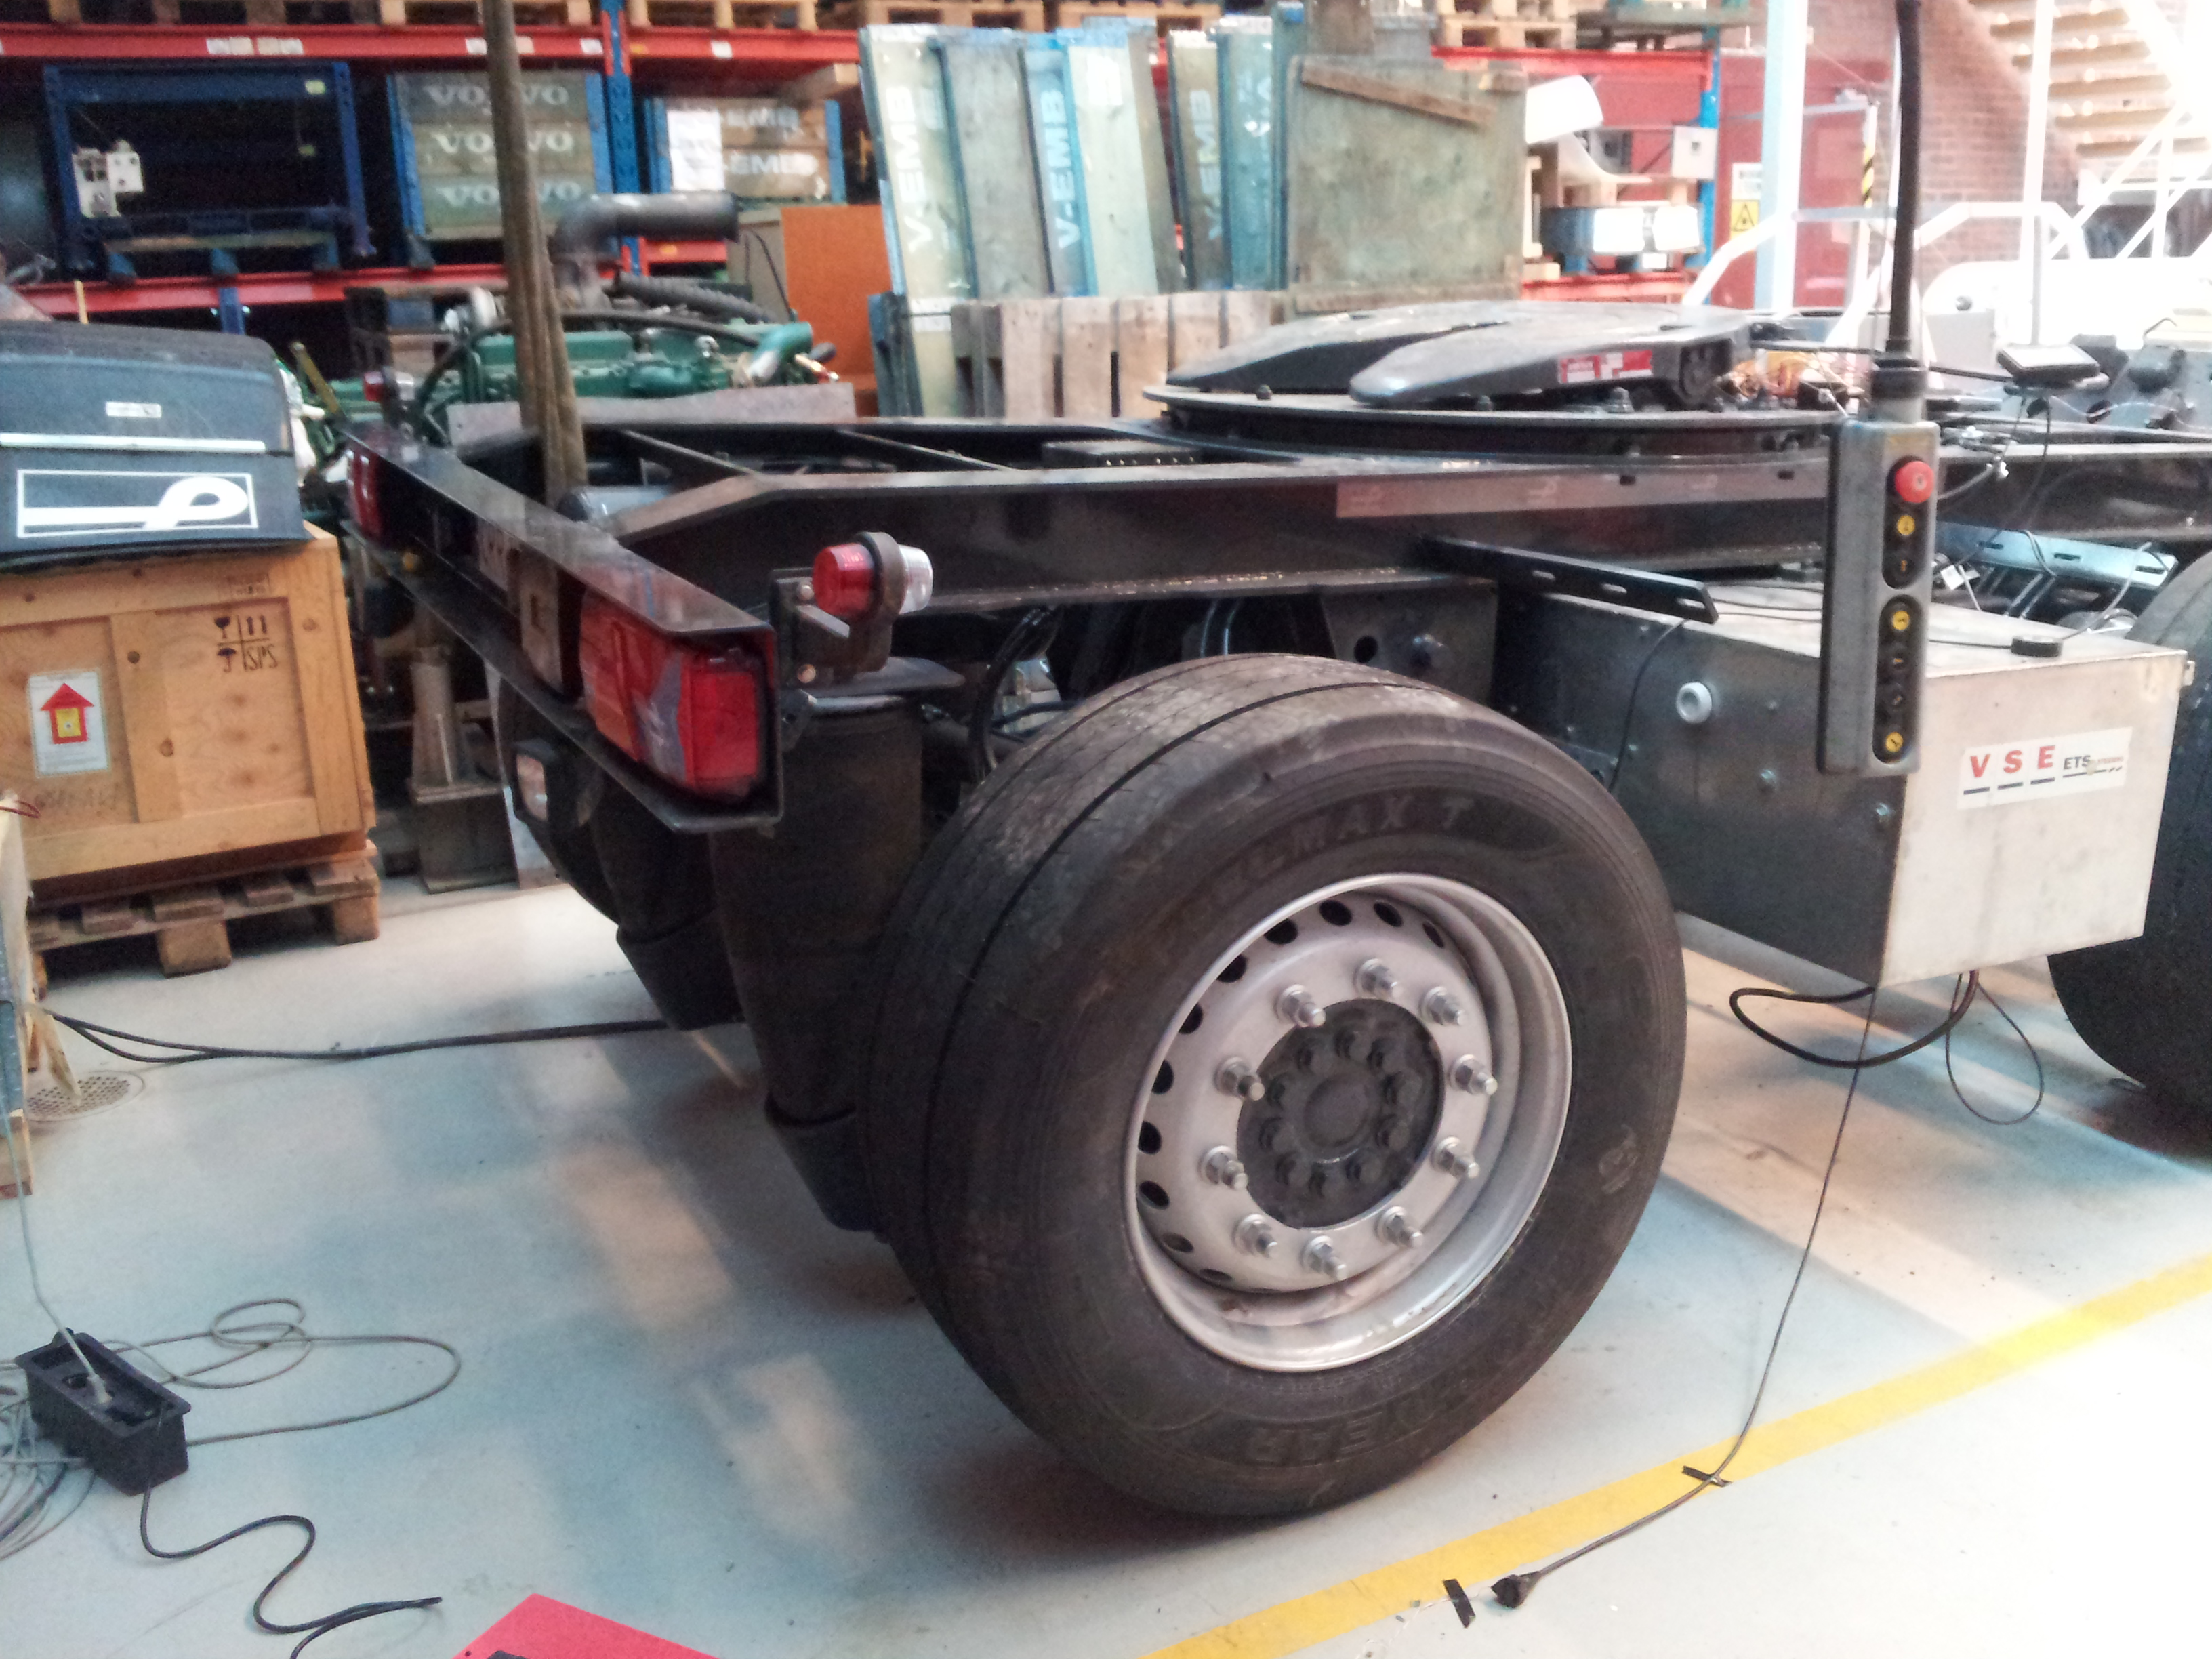
\includegraphics[width=1\linewidth]{figures/dolly_craned_up}
\caption{Dolly craned up slightly to determine delay of steering actuation}
\label{fig:dolly_craned_up}
\end{figure}

\begin{figure}[h]
	\centering
	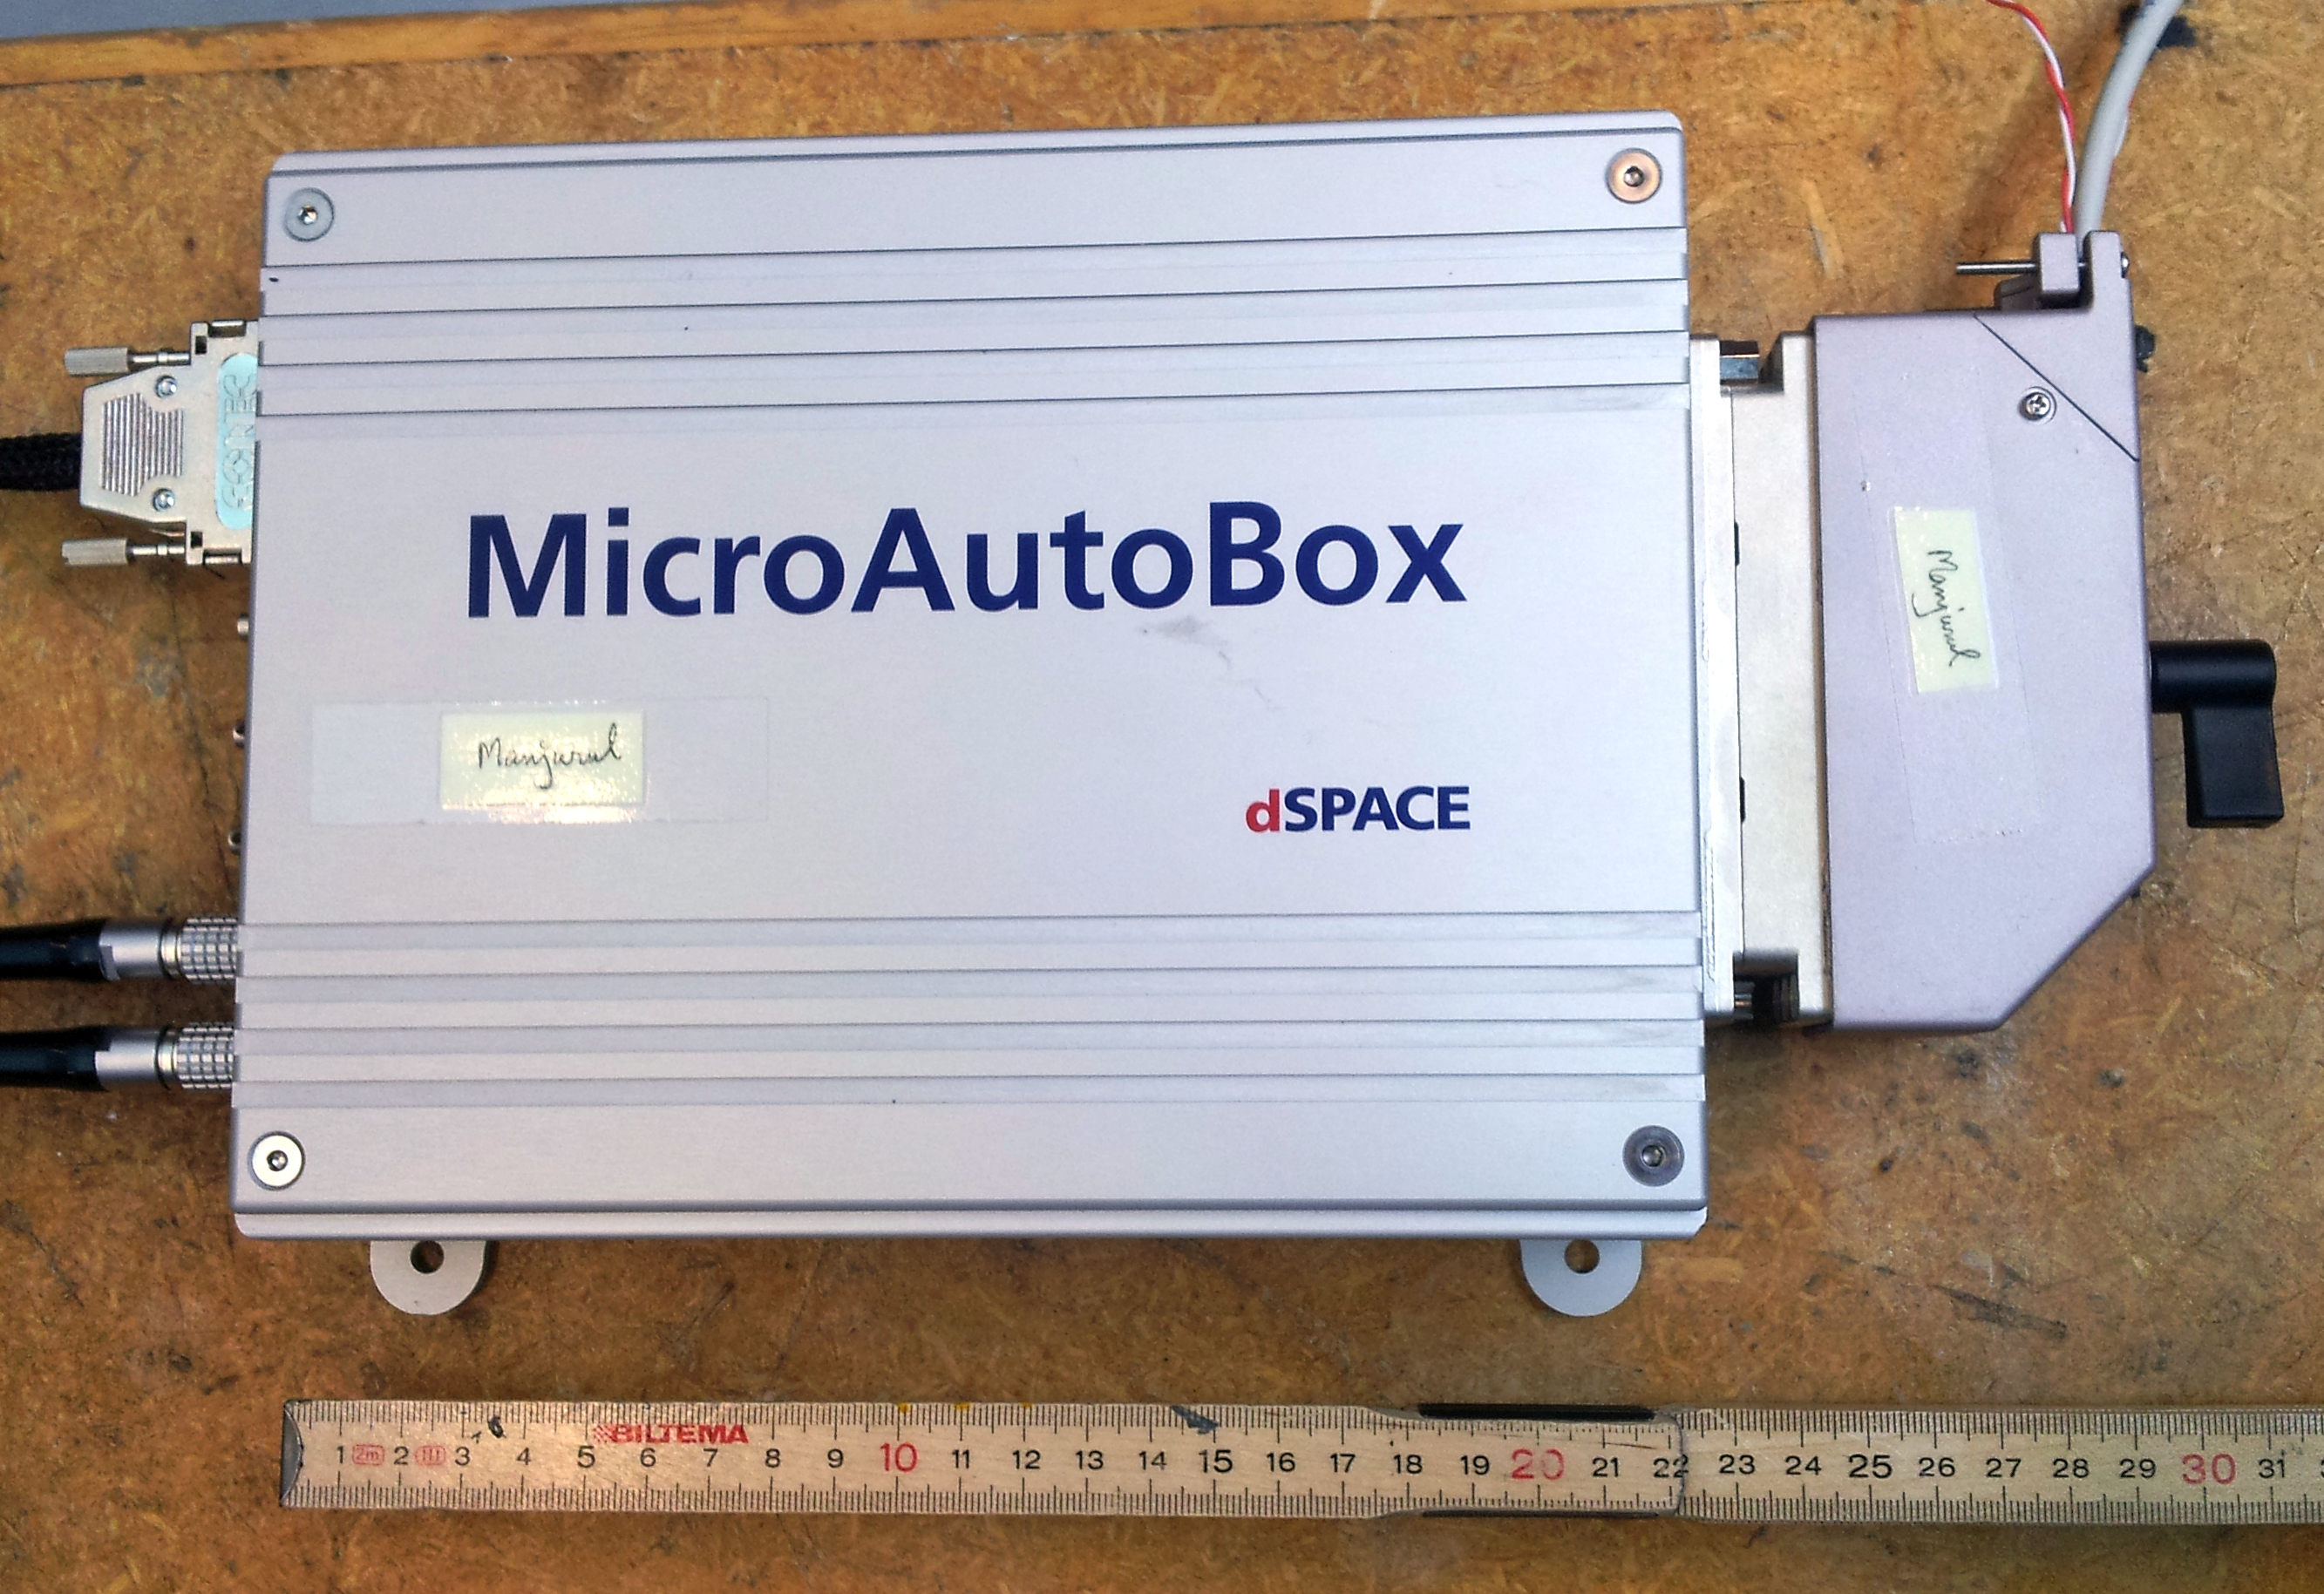
\includegraphics[width=1\linewidth]{figures/MABII_topview_cropped}
	\caption{MicroAutoBoxII viewed from the top including cables for \gls{ZIF} -connector, Host-PC, Simulation-PC and power supply (clockwise, starting on the right)}
	\label{fig:microautobox_topview}
\end{figure}


\begin{figure}[h]
	\centering
	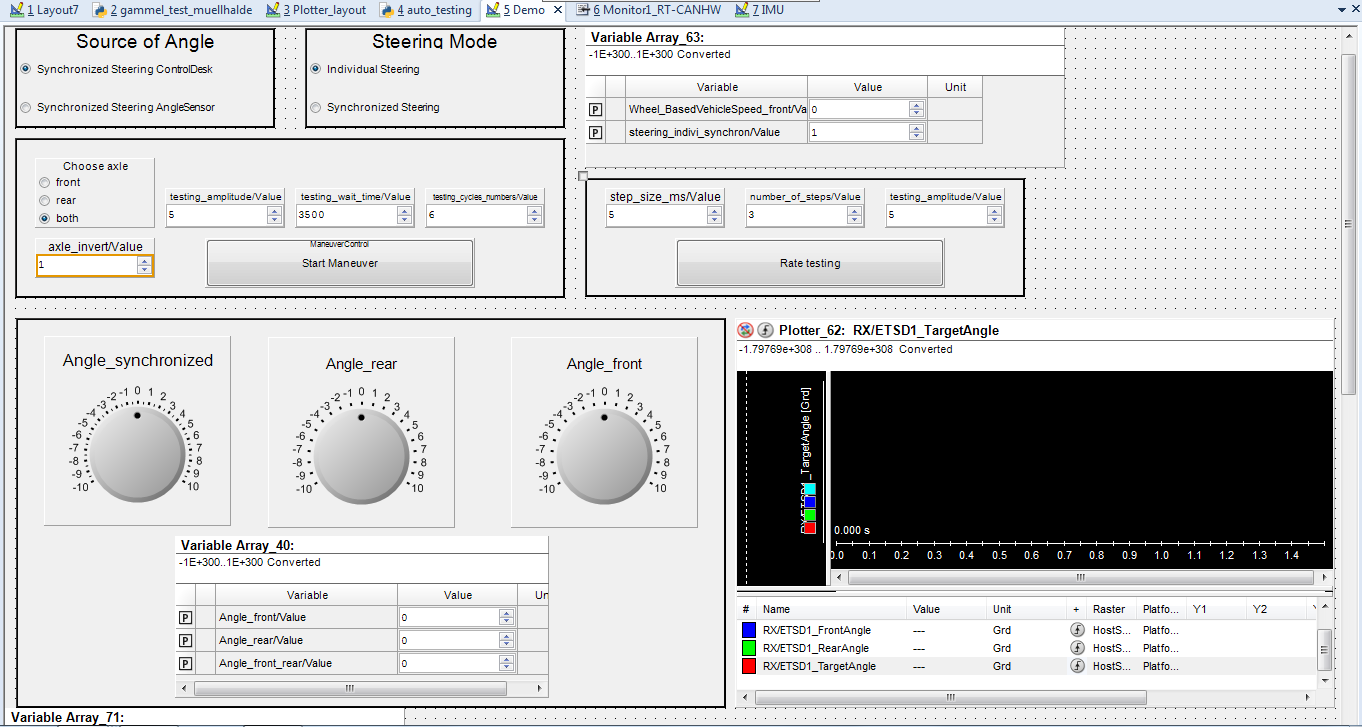
\includegraphics[width=1\linewidth]{figures/CD_Layout}
	\caption{ControlDesk GUI for basic testing and start-up of the dolly}	
	\label{fig:control_desk_GUI}
\end{figure}

\begin{table}[h]
	\centering
	\caption{Severity table for \gls{FMEA} \cite{FMEA_tables}}
	\label{tab:fmea_severity}
	\begin{tabular}{p{4cm}|p{8.5cm}|p{1.5cm}|}
		  Severity & Description & Ranking   \\ \hline
		Hazardous
		without warning     &  Very high severity ranking when a potential failure mode effects safe system operation without warning  & 10        \\
		Hazardous with
		warning   &      Very high severity ranking when a potential failure mode
		affects safe system operation with warning & 9    \\
		Very High &      System inoperable with destructive failure without
		compromising safety & 8       \\
		High&  System inoperable with equipment damage & 7   \\
		Moderate& System inoperable with minor damage & 6  \\
		Low& System inoperable without damage & 5  \\
		Very Low & System operable with significant degradation of
		performance & 4 \\
		Minor & System operable with some degradation of performance & 3 \\
		Very Minor & System operable with minimal interference & 2 \\
		None & No effect & 1 \\
	\end{tabular} \\
\end{table}
\begin{table}[h]
	\centering
	\caption{Probability table for \gls{FMEA} \cite{FMEA_tables}}
	\label{tab:fmea_probability}
	\begin{tabular}{p{8cm}|p{5cm}|p{2cm}|}
		Probability & Description & Ranking   \\ \hline
		Very High: Failure is almost inevitable & \centering \textgreater1 in 2  & 10        \\
		  &   \centering   1 in 3 & 9    \\
		High: Repeated failures &  \centering 1 in 8 & 8       \\
		& \centering 1 in 20 & 7   \\
		Moderate: Occasional failures& \centering1 in 80 & 6  \\
		& \centering1 in 400 & 5  \\
		 & \centering 1 in 2,000 & 4 \\
		Low: Relatively few failures & \centering 1 in 15,000 & 3 \\
		 &  \centering 1 in 150,000 & 2 \\
		Remote: Failure is unlikely &\centering \textless1 in 1,500,000 & 1 \\
	\end{tabular} \\
\end{table}
\begin{table}[h]
	\centering
	\caption{Detectability table for \gls{FMEA} \cite{FMEA_tables}}
	\label{tab:fmea_detectability}
	\begin{tabular}{p{4cm}|p{9cm}|p{2cm}|}
		Detectability & Description & Ranking   \\ \hline
		Absolute Uncertainty & Design control cannot detect potential cause/mechanism and
		subsequent failure mode & 10        \\
		Very Remote &  Very remote chance the design control will detect potential
		cause/mechanism and subsequent failure mode & 9    \\
		Remote &  Remote chance the design control will detect potential
		cause/mechanism and subsequent failure mode & 8       \\
		Very Low & Very low chance the design control will detect potential
		cause/mechanism and subsequent failure mode & 7   \\
		Low &  Low chance the design control will detect potential
		cause/mechanism and subsequent failure mode & 6  \\
		Moderate & Moderate chance the design control will detect potential
		cause/mechanism and subsequent failure mode & 5  \\
		Moderately High & Moderately High chance the design control will detect
		potential cause/mechanism and subsequent failure mode & 4 \\
	High & High chance the design control will detect potential
	cause/mechanism and subsequent failure mode & 3 \\
	Very High	& Very high chance the design control will detect potential
	cause/mechanism and subsequent failure mode & 2 \\
		Almost Certain & Design control will detect potential cause/mechanism and
		subsequent failure mode & 1 \\
	\end{tabular} \\
\end{table}
 






 

  
  
  
 

  
  
 
\end{document}
